% !TEX encoding = UTF-8 Unicode 
% !TEX root = praca.tex

\chapter*{Wprowadzenie}

We współczesnym środowisku medycznym akwizycja i przetwarzanie biosygnałów,  
a w szczególności elektrokardiogramu (\textit{EKG}), stały się nie tylko kluczowym aspektem diagnostyki, 
ale również istotnym elementem monitorowania stanu zdrowia pacjentów \cite{Serhani2020}. 
W obliczu globalnej tendencji wzrostu przypadków zachorowań na przewlekłe choroby układu krążenia, co zostało
wykazane w licznych badaniach \cite{Gaidai2023}, 
obserwuje się zapotrzebowanie na tanie, efektywne oraz szeroko dostępne narzędzia diagnostyczne. 
W tej sytuacji, dostępność tych narzędzi staje się nie tylko wyzwaniem, ale wręcz priorytetem, 
szczególnie w przypadku osób prywatnych oraz w warunkach słabo rozwiniętych 
systemów opieki zdrowotnej \cite{Faruk2021}.

Rozważając wspomniane wyzwania, niezbędnym staje się zwrócenie uwagi na rozwój technologii, które nie tylko zapewnią
efektywną rejestrację i analizę biosygnałów, ale również umożliwią powszechny dostęp do diagnostyki, niezależnie od
wieku, klasy społecznej czy pochodzenia. Poprzez wspieranie szybkiego i skutecznego podejmowania 
decyzji klinicznych,
takie rozwiązania mogą przyczynić się do poprawy jakości opieki zdrowotnej, nawet w trudnych warunkach materialnych.

W ramach niniejszej pracy inżynierskiej, skoncentrowanej na stworzeniu urządzenia 
oraz dedykowanego mu oprogramowania, zaproponowano \textbf{prototyp}\footnote{Urządzenie nie spełnia 
odpowiednich standardów aby być klasyfikowanym jako narzędzie które może być użyte do rozwiązania prawdziwych 
problemów diagnostycznych.} taniego narzędzia diagnostycznego, którego części są powszechnie dostępne. 

Praca ta posiada również wymiar edukacyjny, który wykracza poza aspekty techniczne i inżynieryjne. 
Może ona służyć jako narzędzie do szerzenia świadomości na temat chorób układu krążenia, pomagając zwiększyć zrozumienie ich przyczyn,
symptomów i metod leczenia wśród szerszej publiczności. Dzięki praktycznemu zastosowaniu opracowanego urządzenia i oprogramowania, 
możliwe jest zilustrowanie, jak technologia może przyczyniać się do poprawy diagnostyki i monitorowania zdrowia serca. 
Ponadto, praca ta ma potencjał wykorzystania w edukacji akademickiej i zawodowej, oferując studentom oraz specjalistom inspirację 
do stosowania bardziej praktycznego podejścia do nauki o przetwarzaniu biosygnałów oraz elektroniki. 
Umożliwia to nie tylko głębsze zrozumienie teorii stojącej za tymi dyscyplinami, ale również pozwala na rozwijanie
umiejętności praktycznych poprzez bezpośrednią pracę z urządzeniem, co jest kluczowe w edukacji inżynierskiej i technologicznej.

\newpage

Elektrokardiogram (\textit{EKG}) jest graficznym przedstawieniem aktywności elektrycznej serca, będącej wynikiem jego rytmicznego
skurczu i rozkurczu \cite{Limaye2016}. Sygnał \textit{EKG} jest funkcją napięcia wytwarzanego przez serce, w dziedzinie czasu.
Analiza tego sygnału jest kluczowa dla oceny funkcjonowania serca.
Każdy cykl, obejmujący zarówno fazę skurczu, jak i rozkurczu, reprezentowany jest przez zespół tzw. \textit{załamków} 
oznaczonych literami \textit{P}, \textit{Q}, \textit{R}, \textit{S} i \textit{T}, jak przedstawiono na rysunku \ref{fig:pqrst}.

Jednym z największych wyzwań w systemach akwizycji i przetwarzania sygnałów jest skuteczna eliminacja zakłóceń (\textit{szumów}), 
które w przypadku \textit{EKG} mogą znacząco utrudnić proces diagnostyczny. 
Wśród nich wyróżnić można m. in. \cite{Limaye2016}: dryft linii izoelektrycznej (\textit{baseline wander}), 
szumy pochodzące z instalacji elektrycznych w budynkach (\textit{power line interference}),
a także artefakty spowodowane ruchem pacjenta. Jedną z efektywnych metod eliminacji szumów, jest zastosowanie filtrów cyfrowych, 
w tym filtrów o skończonej odpowiedzi impulsowej \textit{FIR} (\textit{Finite Impulse Response}) \cite{Tompkins1993}.

\begin{figure}[h!]
    \centering
    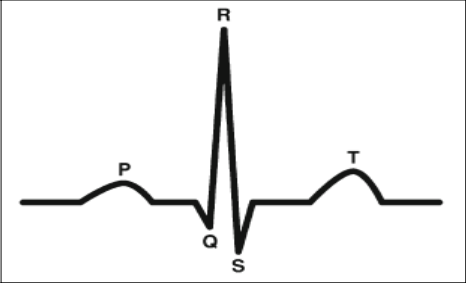
\includegraphics[scale=0.6]{pl/media/pqrst.png}
    \caption{Zespół załamków \textit{PQRST} (\cite{Limaye2016}, fig. 1.)}
    \label{fig:pqrst}
\end{figure}

\newpage

\section*{Cel i zakres pracy}

Celem pracy było stworzenie sprzętowego oraz programowego systemu akwizycji i wstępnego przetwarzania sygnału \textit{EKG} 
mającego znamiona narzędzia diagnostycznego. W zamyśle pracy było stworzenie prototypowego systemu przeznaczonego 
do użytku prywatnego, w tym do wstępnej i samodzielnej oceny stanu mięśnia sercowego a następnie
potencjalnej konsultacji lekarskiej.  
Autor zastrzega jednak, że praca ma wymiar edukacyjny, a celem jej nie było stworzenie narzędzia spełniającego 
standardy urządzenia medycznego.


Niniejsza praca opisuje projekt i realizację dwóch części:

\begin{itemize}

    \item \textbf{sprzętowej}: makieta układu elektronicznego\footnote{Przez makietę rozumiany jest prototyp urządzenia umożliwiającego akwizycję i wstępne przetwarzanie sygnału. }, zawierająca układ wzmacniacza, filtry analogowe, 
    mikrokontroler, programator sprzętowy oraz mostek \textit{USB}/\textit{UART},


    \item \textbf{programowej}: oprogramowanie sprzętowe (inaczej \textit{firmware}), aplikacja na komputery osobiste 
    (zwana w dalszych rozdziałach \textit{aplikacją}) oraz skrypty wspomagające projektowanie filtrów cyfrowych 
    (zwane krócej \textit{skryptami}).

\end{itemize}

Część sprzętowa odpowiada za wstępne wzmocnienie i analogową filtrację sygnału \textit{EKG} 
oraz umożliwienie komunikacji z komputerem osobistym na którym zainstalowana jest wspomniana aplikacja. 


Oprogramowanie sprzętowe (na układ mikrokontrolera makiety sprzętowej) umożliwiło obsługę przetwornika analogowo/cyfrowego,
implementację filtrów cyfrowych oraz implementację protokołu oraz obsługę interfejsu do komunikacji z komputerem osobistym.
Aplikacja na komputery osobiste została stworzona w celu podglądu sygnału oraz jego zapisu w czasie rzeczywistym.

\newpage

\section*{Użyty sprzęt i technologie}

Ze względu prototypowy charakter pracy, część sprzętowa zrealizowana została jako makieta w oparciu o gotowe
płytki drukowane z układami elektronicznymi. W skład części sprzętowej wchodzą następujące elementy, szczegółowiej
opisane w rozdziale 2:

\begin{itemize}

    \item płytka z układem \textbf{AD8232} \cite{AD8232BS} \cite{AD8232ds}: zawiera filtry analogowe oraz układ wzmacniaczy,


    \item płytka z mikrokontrolerem \textbf{STM32F411} oraz programatorem \textbf{STLink v2} \cite{STM32F4DS} \cite{NUCLEO}: 
    zawiera mikrokontroler z mikroprocesorem \textit{ARM Cortex M4} oraz układami peryferyjnymi takimi jak: 
    przetwornik analogowo/cyfrowy, liczniki czy kontroler \textit{DMA} (\textit{Direct Memory Access}),
    

    \item przewody połączeniowe, w tym przewód \textit{USB} do połączenia makiety z komputerem osobistym.


\end{itemize}

W części programowej użyto następujących języków, bibliotek i narzędzi:

\begin{itemize}

    \item \textbf{język C} (standard \textit{C11}): język kompilowany użyty w implementacji oprogramowania sprzętowego,

    \item \textbf{język C++} (standard \textit{C++20}): język kompilowany użyty w implementacji 
    protokołu komunikacyjnego oraz aplikacji,

    \item \textbf{ARM GNU Embedded Toolchain} \footnote{\url{https://developer.arm.com/downloads/-/gnu-rm}}: zestaw narzędzi, w tym
    kompilatorów języków \textit{C} i \textit{C++} oraz \textit{assemblera} dla mikroprocesorów \textit{ARM Cortex-M},

    \item \textbf{biblioteka STM32HAL} \cite{STM32HAL}: biblioteka dostarczająca warstwę abstrakcji dla mikroprocesora 
    oraz układów peryferyjnych mikrokontrolera \textit{STM32F411}.

    \item \textbf{SDL2} \cite{SDL2}: biblioteka umożliwiająca renderowanie rastrowej grafiki dwuwymiarowej zastosowana
    do implementacji wykresu sygnału w aplikacji,

    \item \textbf{standardowe biblioteki języków C i C++ na system GNU/Linux} \cite{GLIBC238}: biblioteki użyte do 
    implementacji komunikacji międzyprocesowej, wielowątkowości oraz niektórych struktur danych w aplikacji,

    \item \textbf{CMake} \footnote{\url{https://cmake.org/}} \textbf{oraz GNU Make} 
    \footnote{\url{https://www.gnu.org/software/make/}}: systemy automatyzujące 
    kompilację i konsolidację aplikacji w językach \textit{C} i \textit{C++},

    \item \textbf{język Python 3} \cite{python}: język skryptowy użyty do napisania 
    skryptów obliczeniowych i pomocniczych w projektowaniu filtrów cyfrowych,
   
\item biblioteki \textbf{SciPy}, \textbf{NumPy}, \textbf{matplotlib}
    \cite{SciPy} \cite{NumPy} \cite{matplotlib}: biblioteki języka \textit{Python} użyte w pracy 
    do obliczeń, zaprojektowania filtrów cyfrowych i wizualizacji danych na wykresach.

\end{itemize}

